\DontNumberThisInToc
\DontFrameThisInToc
\glsresetall
\ChapterNumberCitation{Le Système Visuo-moteur}{Perception is not something that happens to us, or in us, it is something we do.}{ N. Alva, Action in Perception, 2006}{10cm}
\Citation {During visual search, the brain
performs a sophisticated deployment
of eye movements (\protect\textit{saccadic actions})
to gather information to subserve
perceptual judgments}
{P.E Miguel et al., J. Neuroscience, 2007}{10cm}
\section{Introduction}

Les images visuelles perçues par nos yeux sont une source riche d'informations sur le monde extérieur. Notre système visuo-moteur est capable d'analyser avec précision ces informations, les acheminer correctement vers les régions du cerveau impliquées dans la perception, la planification et le contrôle moteur. Par exemple, lors d'une tâche habituelle comme conduire sa voiture, nous avons besoin de coordonner plusieurs tâches visuelles: la reconnaissance de la route, la lecture des panneaux, les feux, la lecture du tableau de bord, la localisation des véhicules, des piétons et la vigilance par rapport aux dangers. Notre capacité à coordonner de telles tâches rapidement et efficacement dans notre environnement naturel nécessite un système visuel extrêmement sophistiqué.\\

Cependant, il nous est difficile de traiter toutes les informations visuelles que nous sommes susceptibles de recevoir de notre environnement. Il est impératif de choisir des points d'intérêt particuliers à considérer. La question de savoir quelles informations sont récupérées par le système perceptif au cours et grâce à ces mouvements nous intéressera par la suite. Habituellement, les mouvements des yeux déplacent le regard vers des stimuli saillants dans le champ visuel qui attirent notre attention. \\

Ces mouvements oculaires semblent être les mouvements les plus simples à étudier. Au niveau musculaire, l'oeil peut être mobilisé dans différentes directions grâce à seulement six muscles striés (quatre muscles droits et deux muscles obliques), sous l'influence de l'innervation des nerfs oculomoteurs (fig.\ref{oeil}). Ils agissent pour tourner ou pivoter un œil autour de ses axes verticaux, horizontaux, et antéro-postérieur:\\

\begin{itemize}
\item le muscle droit médian déplace le regard vers l'intérieur, vers le nez (adduction).
\item le muscle droit latéral déplace le regard vers l'extérieur, loin du nez (abduction).
\item le muscle droit supérieur déplace principalement le regard vers le haut (élévation). Il permet de tourner la partie supérieure de l'oeil du côté du nez (intorsion) et aide à déplacer l'oeil vers l'intérieur (adduction).
\item le muscle droit inférieur déplace le regard vers le bas (dépression). Il permet aussi de tourner la partie supérieure de l'oeil loin du nez (extorsion) et aide à déplacer l'oeil vers l'intérieur (adduction)
\item le muscle oblique supérieur tourne essentiellement le haut de l'oeil vers le nez (intorsion), déplace l'oeil vers le bas (dépression) et vers l'extérieur (enlèvement).
\item le muscle oblique inférieur tourne essentiellement le haut de l'oeil loin du nez (extorsion), déplace le regard vers le haut (élévation) et vers l'extérieur (abduction)\\
 \end{itemize}

\begin{figure}
\begin{center}
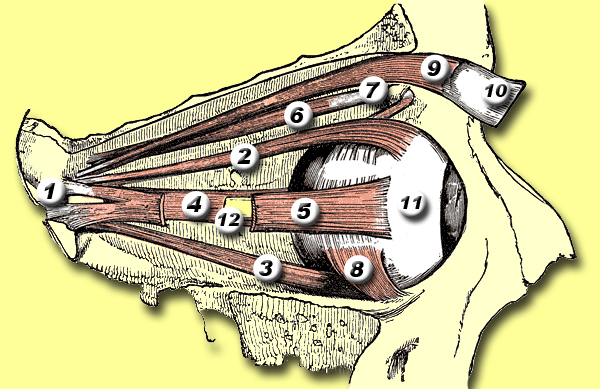
\includegraphics[width=6cm]{figures/ch2_1_oeil}
\end{center}
\caption{ Disposition des muscles oculomoteurs de l'oeil droit: 1=Tendon de Zinn, 2= Muscle droit supérieur, 3=Muscle droit inférieur, 4=Muscle droit médian, 5=Muscle droit latéral, 6=Muscle oclique supérieur, 7=Muscle oblique inférieur, 9=Élévateur de la paupière, 10=Paupière, 11=Globe oculaire, 12=Nerf optique.[Wikipedia]}
\label{oeil}
\end{figure}

Plusieurs résultats sur la régulation des mouvements par le cervelet, les ganglions de la base et le système vestibulaire se sont basés sur les mouvements des yeux \cite{Purves:2005} comme modèle basique d'intégration sensori-motrice. Dans ce chapitre, nous passerons en revue les différents types de mouvements oculaires ainsi que leur intérêt et leur utilisation dans différentes tâches, en s'intéressant en particulier aux mouvements saccadiques (les saccades) visuellement guidés. Il s'agit de mouvements rapides et précis du globe oculaire qui permettent de modifier la direction du regard vers un nouveau point d'intérêt.\\

En plus des études électrophysiologiques sur les singes, l'imagerie fonctionnelle et la stimulation magnétique transcrânienne chez les humains, ont permis d'identifier plusieurs zones corticales et sous corticales qui contribuent à la programmation des saccades \cite{Pierrot:2002}. Nous donnerons une description générale des principales structures, ainsi que les hypothèses sur leurs rôles.\\

Enfin, le système saccadique représente un site d'intégration sensori-motrice. Les stimuli lumineux se projettent sur la rétine produisant des modifications physiques et chimiques dans les récepteurs rétiniens. Ces modifications des changements d'activité des neurones et les signaux représentant cette information visuelle reçue seront transmis au système nerveux central sous forme d'impulsions. Ensuite, une fois cette information traitée, une réponse motrice est ordonnée aux muscles agissant sur les globes oculaires. C'est ainsi qu'on considère que le système moteur est au service du système sensoriel par lequel il est régi. Nous examinerons les aspects d'intégration visuo-motrice dans la troisième section de ce chapitre. \\

Mais avant cela, un rapide survol de l'anatomie de l'oeil est nécessaire.\\

\section{L'anatomie oculaire : la rétine}

L'anatomie du système visuel des primates a été intensivement étudiée chez le singe macaque étant donné sa ressemblance avec celui de l'Homme (pour une revue voir \cite{Leigh:2004}). L'oeil capte les rayons lumineux, l'information est transmise aux aires visuelles via le nerf optique. La partie de l'oeil sensible à la lumière est la rétine. Il s'agit d'une mince surface d'environ $0,5 mm$ d'épaisseur située au fond de chaque oeil, couvrant $3/4$ du globe oculaire. Elle possède une structure complexe composée de couches successives de neurones (figure \ref{Ret}). La couche la plus externe est adhérente à la choroïde, qui est une couche vasculaire de couleur noire qui tapisse les trois cinquièmes postérieurs du globe oculaire. Elle absorbe les rayons lumineux inutiles pour la vision et nourrit les photo-récepteurs de la rétine grâce à sa richesse en vaisseaux sanguins. Les premiers phénomènes de la vision débutent dans la couche de photorécepteurs (cônes et bâtonnets) qui compte environ $130$ $millions$ bâtonnets sensibles à la lumière faible et assurent la vision nocturne et $65$ $millions$ de cônes qui répondent à une luminosité intense, permettent la vision des couleurs et la distinction des détails \cite{Gregory:2000, Sekuler:1990}.\\ 

\begin{figure}[h]
\begin{center}
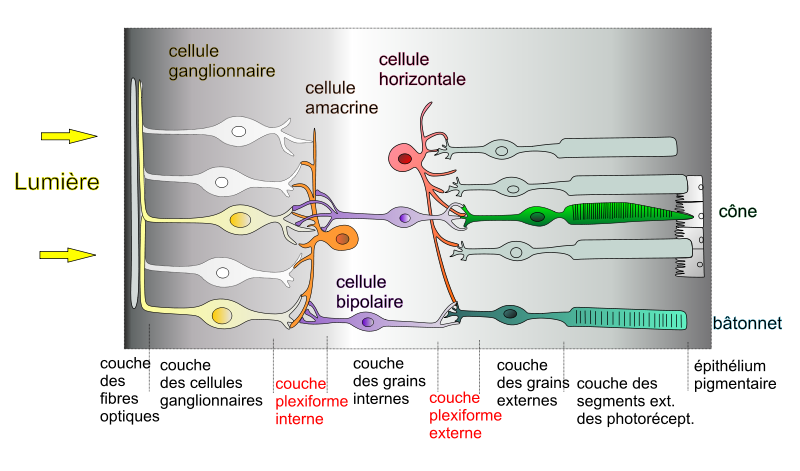
\includegraphics[width=17cm,height=10cm]{figures/ch2_2_Retina}
\end{center}
\caption{ Structure de la rétine : La couche monostratifiée des cellules photoréceptrices glutaminergiques (les cônes au sein de la fovéa, ou les bâtonnets plus en périphérie). La couche plexiforme externe formée des cellules horizontales de type H1 et H2. La couche nucléaire interne (ou couche des grains internes) formée des cellules bipolaires GABAergiques et glycinergiques, de plusieurs types (les cellules bipolaires périphériques, spécifiques des bâtonnets, et les cellules bipolaires centrales, spécifiques des cônes, lesquelles comptent au moins les sous-classes suivantes : géantes, diffuses, midget et S-cône). La couche plexiforme interne formée des cellules amacrines. La couche des cellules ganglionnaires dont les axones se connectent de façon excentrée au niveau de la macula (comprenant moins de couches et dépourvue de cellules photosensibles) pour donner le nerf optique [Wikipedia].}
\label{Ret}
\end{figure}

%%%%%%%%%%%%%%%%%%%%%%
Ensuite, le flux nerveux est transmis jusqu'aux cellules ganglionnaires qui sont les neurones de sortie de la rétine chez les vertébrés. Elles reçoivent les informations sur le monde visuel via des cellules bipolaires et des cellules amacrines (interneurones rétiniens). Mais à la différence des photorécepteurs qui répondent à la lumière par un changement du potentiel de membrane, ces cellules transmettent l'information visuelle sous forme de potentiels d'action. Elles sont activées de manière permanante même en l'absence de lumière mais leur activité tonique est modulée par les signaux d'entrée provenant des neurones rétiniens. Tout comme les neurones des différentes couches de la rétine, chaque cellule ganglionnaire couvre une région de notre champ visuel\footnote{Le champ visuel est défini par la partie de l'espace que l'oeil immobile peut voir autour du point qu'il fixe. On distingue le champ visuel monoculaire (exploré en clinique) du champ visuel binoculaire correspondant à la superposition par la partie nasale des deux champs monoculaires. Les limites périphériques d'un champ visuel normal varient selon le secteur: $90°$ à $110°$ dans le champ temporal, $60°$ à $90°$ dans le champ nasal, $60°$ dans le champ supérieur et $75°$ dans le champ inférieur. Le passage des rayons lumineux émanant d'un objet, à travers les milieux transparents de l'oeil, inverse les images des objets du champ visuel sur la surface de la rétine, dans le sens bas-haut et droite-gauche. Les objets de la partie temporale sont vus par le champ rétinien nasal et ceux de la partie supérieure du champ visuel par le champ rétinien inférieur \cite{Flament:2002}.} appelée le champ récepteur de ce neurone, c'est à dire que la présence d'un stimulus approprié dans cette région modifie l'activité nerveuse de cette cellule. Le champ récepteur des cellules ganglionnaires est très petit au centre de la rétine et devient de plus en plus grand vers la partie périphérique.\\

En effet, dans la rétine, l'acuité visuelle\footnote{Elle est définie comme la capacité à distinguer les plus fins détails spatiaux de haut contraste.} décroît du centre de la rétine (\textit{la fovéa} qui est la partie centrale de la macula\footnote{La macula est la zone de la rétine caractérisée par une concentration maximale de cônes. Située au fond de l'oeil, la macula a un diamètre d'environ $2$ $mm$. La macula contient en son centre une petite dépression appelée la fovéa : entièrement composée de cônes serrés les uns contre les autres, celle-ci est la zone d'acuité maximale de l'oeil [wikipedia]}) vers la périphérie. Cette propriété est attribuée à une variation de la densité des photo-récepteurs qui décroît du centre à la périphérie \cite{Marilly:1999}. 

\begin{figure} [htbp]
\begin{center}
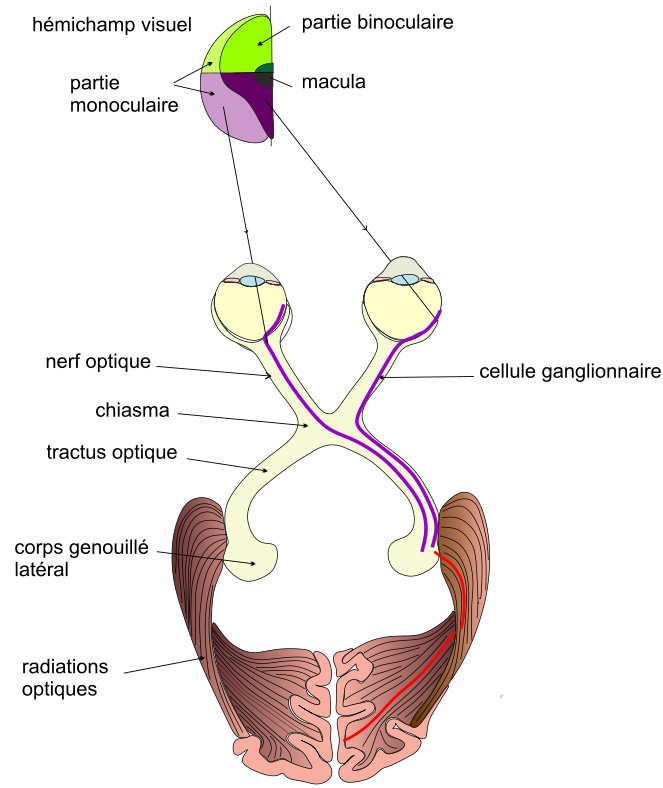
\includegraphics[width=10cm,height=12cm]{figures/ch2_3_Voies}
\end{center}
\caption{Le chiasma optique permet la \textit{décussation} d'un certain nombre d'axones en provenance de la rétine pour assurer le traitement croisé de l'information visuelle. C'est donc le lieu du rassemblement des informations visuelles d'un même hémichamp (demi-champ) visuel captées par les deux rétines. La grande majorité des fibres nerveuses du tractus optique projette sur le corps genouillé latéral dans la partie dorsale du thalamus, le relais principal de la voie qui mène au cortex visuel primaire [Wikipedia]. }
\label{Dec}
\end{figure}

La fovéa est définie donc comme la région o\`u l'acuité visuelle est maximale, ses champs récepteurs se trouvent au centre du champ visuel. On distingue donc la vision centrale (centrée sur la fovéa) qui permet une bonne qualité d'analyse de formes et de couleurs en termes de précision, de la vision périphérique plus efficace dans la détection de mouvements. Les connexions entre les différentes cellules de la rétine centrale sont unitaires (Chaque cône n'y est connecté qu'à une cellule bipolaire, elle même liée qu'à une cellule ganglionnaire). Par contre au niveau de la rétine périphérique, les connexions sont convergentes puisque la densité des cônes diminue considérablement par rapport au nombre de cellules ganglionnaires (plusieurs récepteurs sont connectés à chaque cellule ganglionnaire) et l'acuité est corrélativement fortement réduite. L'organisation des circuits nerveux rétiniens implique donc que la rétine centrale (fovéa) est plus discriminative (reconnaissance de l'information) que la rétine périphérique. Par contre cette dernière est beaucoup plus sensible (détection de l'information).\\



Enfin, les axones des cellules ganglionnaires se rassemblent pour constituer le nerf optique \cite{Purves:2004} qui projette vers les centres visuels du cerveau, principalement le corps genouillé latéral du thalamus et le colliculus supérieur (décrits dans la suite). Les nerfs optiques se réunissent pour former \textit{le chiasma optique} juste en avant de l'hypophyse. Le chiasma optique permet le changement de côté d'un certain nombre d'axones (du coté nasal) en provenance de la rétine  pour assurer le traitement croisé de l'information visuelle (fig \ref{Dec}). Ces axones vont changer de côté au niveau du chiasma optique pour faire en sorte que la moitié gauche du champ visuel soit perçue par l'hémisphère cérébral droit, et vice-versa.\\%Décussation

Les informations visuelles sont ensuite traitées corticalement. Suite aux travaux de \cite{Ungerleider:1982}, on distingue fonctionnellement deux grandes voies de traitement cortical de l'information visuelle : la voie \textit{ventrale}, celle de l'identification des objets et la voie \textit{dorsale}, celle de la localisation des objets et la préparation de l'action. Leurs descriptions seront détaillées plus loin dans le texte. Nous allons nous intéresser plus à la voie dorsale qui traite les informations liées aux mouvements des yeux et le contrôle visuel de l'action pour permettre en particulier les mouvements en direction ou non des objets présents. On commencera donc par passer en revue les différents types de mouvements oculaires puis une description fonctionnelle des différentes strutures corticales et sous-corticales impliquées dans l'encodage de ces mouvements sera donnée. 

\section{Les mouvements oculaires}

Ces mouvements de rotations que les globes oculaires effectuent autour de leurs centres modifient la direction de la ligne de regard. Ils servent à explorer les scènes visuelles, à réagir à l'apparition de nouveaux objets, à suivre des objets mobiles. Ils peuvent être volontaires (recherche d'un élément dans l'environnement) ou réflexes (compensation des mouvements de la tête). On distingue les mouvements effectués par un seul oeil, dits \textit{mouvements de duction}, des mouvements simultanés des deux yeux qui permettent une vision binoculaire. Les deux yeux peuvent bouger, soit de manière identique, on parle donc de \textit{mouvements de version} (ou mouvements conjugués), soit de manière symétrique, on parle alors de \textit{mouvements de vergence}. \\

La plus ancienne classification fonctionnelle des mouvements des yeux date de 1903 \cite{Dodge:1903}. Dodge et Cogan étaient les premiers à distinguer \textit{les saccades oculaires} des autres mouvements des yeux (poursuite lente, vergence, réflexe optocinétique, réflexe vestibulo-oculaire). Les catégories oculomotrices décrites à l'époque sont encore en usage aujourd'hui. Nous nous sommes intéressés dans nos travaux aux saccades et pour bien situer ce type de mouvements nous donnons dans la suite une revue des différents mouvements chez le primate. \\
 

\subsection{Les mouvements de stabilisation}

Il s'agit de mouvements oculaires qui agissent en synergie pour permettre une vision nette et centrale quand le corps est mobile ou quand l'objet visionné est mobile. Les trois classes de mouvements de yeux qui opèrent dans la même gamme de vitesses sont: la poursuite lente, le nystagmus optocinétique qui consiste en une alternance entre des mouvements oculaires rapides et lents provoquée par un grand champ de mouvement visuel et le réflexe vestibulo-oculaire qui stabilise le regard lors des mouvements de la tête. \\

Chez les primates ayant une région fovéale, les mouvements oculaires de poursuite lente (\textit{smooth poursuit}) permettent de suivre de près un objet en mouvement sans que l'image de l'objet ne s'écarte de la fovéa. Lorsque le mouvement de poursuite est bien développé, il s'effectue de façon continue, lente, fluide et régulière, sans changements brusques de points de fixation (voir \cite{Leigh:1999, Ilg:1997} pour un aperçu). Ils sont exécutés volontairement mais la plupart des gens sont incapables d'initier un mouvement de poursuite sans un signal visuel en mouvement. En outre, la poursuite de cibles mobiles avec des vitesses supérieures à $30°/s$ nécessite souvent des mouvements de rattrapage. \\

Ce type de mouvement n'existe que chez les primates \cite{Buttner:1988} et se distingue du réflexe opto-cinétique (\textit{optokinetic nystagmus}) commun à tous les mammifères. Le réflexe opto-cinétique réagit aux mouvements d'ensemble du champ visuel, alors que la poursuite opère sur une petite région. Ce reflexe consiste en deux phases. D'abord, une phase lente avec de lisses mouvements oculaires de compensation dans la direction du mouvement. Ensuite, une phase rapide avec des mouvements dans la direction opposée à la phase lente pour repositionner les yeux dans les plus brefs délais comme dans le cas de suivi des arbres à travers les fenêtres d'un train en mouvement. Il permet donc de réajuster le regard suite à une rotation prolongée et dirige le regard vers la cible à venir.\\

Il se distingue aussi du réflexe vestibulo-oculaire qui est indépendant de la stimulation visuelle et est provoqué par des mouvements de tête, même dans l'obscurité. Il permet de stabiliser la position des yeux par rapport au monde extérieur et compense donc les mouvements de la tête pour maintenir l'image de l'environnement stable sur la rétine pendant les rotations brèves de la tête. Une vision claire lors de la marche, par exemple, n'est possible que parce que le réflexe vestibulo-oculaire est assez rapide pour générer des mouvements oculaires compensatoires\cite{Grossman:1988}. \\

Avec ces mouvements, les primates peuvent suivre activement des objets en mouvements avec leurs yeux et peuvent aussi garder les yeux sur des objets fixes lorsque la tête ou le corps entier bouge. Ces mouvements oculaires lents coexistent et sont souvent utilisés en conjonction pour stabiliser le regard et interagir avec les objets dans un environnement dynamique \cite{Leigh:1987,Paige:1983,Yee:1983}.\\

\subsection{Les mouvements de vergence}

La vergence est le mouvement simultané des deux yeux dans des directions opposées tout en maintenant une vision binoculaire \cite{Cassin:1990}. Les deux yeux convergent pour voir une cible plus proche et divergent pour fixer une cible plus éloignée. Le système de vergence se développe pendant les trois premiers mois du nourrisson et se dégrade à partir de la cinquantaine. \\

Les mouvements de vergence sont principalement provoqués par une disparité entre les images des deux yeux. La disparité vient du fait qu'une image se projette sur des emplacements différents sur les deux rétines. Ceci provoque une diplopie, c'est à dire la perception d'une image double. La fusion des images rétiniennes des deux yeux est possible même si les images ne sont pas exactement confondues. On appelle aire de Panum l'aire dans laquelle deux images rétiniennes fusionnent pour donner une unique perception. La taille de cette aire dépend des personnes et de l'excentricité de la cible. Elle est de l'ordre d'une dizaine de minutes d'arc au niveau de la fovéa et peut aller jusqu'à $40$ $minutes$ $d'arc$ en excentricité.\\


Les mouvements de vergence sont de petite amplitude, de l'ordre de quelques degrés, environ $3°$ par oeil. Les temps de réaction sont de $160$ $ms$ à $200$ $ms$ et la vitesse de l'ordre de $25\degres/s$. Outre les mouvements de convergence ou divergence, il existe aussi une activité de vergence tonique qui maintient les yeux au repos avec un certain angle de vergence. Cette vergence de repos dépend de l'orientation des yeux dans les globes. \\

\subsection{Les mouvements saccadiques}

Les saccades oculaires sont des mouvements rapides et précis du globe oculaire permettant de modifier la direction du regard vers un nouveau point d'intérêt (de fixation). Ces mouvements brusques placent l'image du point de fixation de la scène visuelle sur la \textit{fovéa} ($1.5 mm$ de diamètre), assurant ainsi une intégration et une analyse plus fine de l'information visuelle (processus de fovéation).\\

La durée des saccades varie entre $20$ et $200$ $ms$. Cette durée dépend en particulier de l'\textit{amplitude du mouvement saccadique}: la distance angulaire que l'oeil doit survoler pendant le mouvement. Les relations stéréotypées entre la durée et l'amplitude d'une saccade, d'une part, et entre la vélocité maximale d'une saccade et son amplitude, d'autre part, sont connues sous le terme de séquence principale de la saccade (\textit{saccadic main sequence} \cite{Bahill:1975}). Pour des amplitudes comprises entre 4° et 40°, la durée d'une saccade dépend presque linéairement de son amplitude et la vélocité maximale dépend logarithmiquement ou exponontiellement de l'amplitude \cite{Becker:1991,Garbutt:2001}.\\ %Cette amplitude va des déplacements de petite taille (lors de la lecture par exemple) jusqu'aux 4 coins d'une pièce. vitesse angulaire maximale 1000°/s
 
Les mouvements saccadiques forment une hiérarchie en partant des saccades les plus élémentaires (saccades réflexes) en réponse à des apparitions soudaines d'objets dans le champ visuel pour arriver au niveau supérieur (saccades vers des positions mémorisées après disparition de stimuli) \cite{Leigh:1999}. On peut les classer selon leur objectif comme suit :\\
\begin{itemize}

\item[$\bullet$]{\em les saccades volontaires} sont des saccades sélectionnées dans le cadre d'un comportement intentionnel. Elles sont réalisées suite à une consigne ou une décision prise en interne de déplacement du regard vers un objet (ou une cible) déjà présent dans l'environnement visuel de la personne.\\

\item[$\bullet$]{\em les saccades réflexes} se déclenchent de manière exogène par l'apparition d'un stimulus périphérique, ou par la disparition d'un stimulus de fixation. Dans les conditions naturelles, nous faisons plusieurs saccades spontanées par seconde. Elles peuvent être déclenchées par un stimulus visuel, auditif ou somesthésique.\\

\item[$\bullet$]{\em les saccades prédictives ou anticipées} servent à anticiper la recherche d'une cible, un objet ayant un mouvement régulier. Elles sont réalisées en anticipation de l'apparition d'un objet ou d'une cible.\\


\item[$\bullet$]{\em les saccades guidées par mémorisation} sont des saccades vers une position mémorisée d'un stimulus présenté dans le passé. Il s'est avéré utile d'étudier la précision de ces saccades, en particulier chez les patients présentant des lésions affectant les lobes frontaux et les noyaux gris centraux qui pourraient nuire à la mémoire de travail. Lorsque les sujets normaux tentent de faire des saccades à l'emplacement d'une cible mémorisée qu'ils fixaient quelques secondes avant, ils le font avec un peu moins de précision que si la cible était visible.\\

\item[$\bullet$]{\em les antisaccades} sont des saccades qui éloignent les yeux du stimulus visuel. Une antisaccade réussie nécessite l'inhibition d'une saccade réflexe vers l'endroit du stimulus, et le déplacement volontaire de l'oeil dans la direction opposée. En plus de regarder vers de nouvelles cibles visuelles, une partie importante du comportement saccadique est de supprimer les mouvements oculaires qui seraient apportées vers les nouveaux stimuli qui ne sont pas importants (perturbateurs). Pour étudier un tel contrôle des saccades volontaires par rapport aux réflexes, un paradigme de test spécial est appelé la tâche antisaccade. 
Dans cette tâche, il est nécessaire de supprimer une saccade vers un stimulus qui apparaît dans la périphérie de la vision pour générer une saccade volontaire de taille égale vers le côté opposé \cite{Fischer:1997}. La mesure la plus simple de la réponse à ce test concerne la direction de la saccade initiale \cite{Currie:1991}. Les sujets normaux font d'abord beaucoup d'erreurs sur cette tâche, mais après une brève période de pratique, le taux d'erreur baisse à moins de 15\%.\\

\item[$\bullet$]{\em les saccades spontanées} sont des saccades aléatoires involontaires qui peuvent être réalisées même dans l'obscurité.\\

\item[$\bullet$]{\em les micro-saccades} sont des mouvements minuscules, environ $20$ secondes d'arc et sont complètement imperceptibles en temps normal. En effet, même lors de la fixation d'un objet, l'oeil humain est dans un état constant de vibration, oscillant dans plusieurs sens à un taux d'environ $60$ vibrations par seconde. Ces micro saccades servent à rafraîchir l'image  projetée sur les cellules bâtonnets et les cellules cônes à l'arrière de l'oeil. Sans micro-saccades, regarder fixement quelque chose causerait la cessation de la vision après quelques secondes puisque les bâtonnets et les cônes répondent seulement à un changement de luminosité \cite{Pettigrew:1990}.\\

\end{itemize}
%(figure Metriques d'une saccade oculaire d'après fuchs 1967).

Il est également utile de classer les saccades selon la \textit{latence} (le temps entre l'apparition du stimulus visuel et le déclenchement du mouvement). Dans ce cas, la catégorisation est binaire: une saccade donnée est une saccade ``express'' ou elle ne l'est pas. Le temps de latence de référence est d'environ $~100 ms$. S'il est dépassé, il ne s'agit pas de saccades express. Ces saccades express sont générées par un mécanisme neuronal qui contourne les longs circuits et active les muscles de l'oeil plus directement \cite{Fischer:1983}. Il s'agit du chemin sous-cortical qui part de la rétine vers la formation réticulée en passant par le colliculus supérieur.\\

Il en résulte donc que les saccades sont caractérisées principalement par les grandeurs suivantes : la direction, l'amplitude, la vitesse et la latence. Nous aborderons dans la section suivante la description des structures corticales et sous-corticales qui participent en particulier à la génération des saccades, et plus généralement à l'intégration visuo-motrice.

\section{Les structures corticales et sous corticales impliquées dans la gestion des saccades}


Reprenons l'exemple de la conduite d'une voiture. Après avoir reçu l'information visuelle (un panneau de signalisation lumineux, feux, clignotant...) dans le lobe occipital (le cortex visuel) du cerveau du conducteur, l'intégration visuo-spatiale est assurée dans le lobe pariétal plus particulièrement dans le cortex pariétal postérieur (position relative, vitesse, ...). Une saccade peut être déclenchée soit par réflexe (suite à un signal lumineux brusque), principalement par le biais du champ oculaire pariétal, ou intentionnellement (pour lire un panneau par exemple) impliquant les champs oculaires frontaux, une zone qui semble également être impliquée dans la fixation visuelle active (les micro-saccades).\\

Si une saccade réflexe doit être inhibée (faire une saccade vers le rétroviseur à gauche et non pas vers une signalisation à droite), on passe donc au lobe frontal, le cortex préfrontal dorsolatéral semble y participer. Cette zone est également impliquée dans la mémoire spatiale à court terme et la prédiction, donc elle est fortement stimulée lors d'une tâche de navigation. Elle assure un rôle important dans les processus décisionnels de contrôle du comportement oculomoteur. En outre, les champs oculaires frontaux pourraient être stimulés puisqu'ils sont impliqués dans les contrôles de haut niveau tels que les transformations spatiales, les mouvements appris et l'ajustement des programmes moteurs. Ces régions corticales interagissent ensuite avec d'autres structures sous-corticales pour préparer l'exécution des mouvements.\\

En particulier, le colliculus supérieur code l'amplitude et la direction des saccades volontaires en se basant sur la position du stimulus (visuel: panneau ou auditif: klaxon). L'activation de cette structure est modulée par l'action d'un ensemble de noyaux sous-corticaux appelés les ganglions de la base impliqués dans la sélection de l'action. Cette structure est fortement sollicitée lors de la phase de l'apprentissage (ce qu'il faut regarder en premier avant de s'arrêter ou avant de s'insérer dans une voie rapide...). Les décisions motrices sont ensuite envoyées à la formation réticulée qui contient les centres vertical et horizontal du regard. Cette structure envoie les commandes de déclenchement de saccades vers les neurones moteurs qui innervent les muscles extra-oculaires. Ces ordres moteurs sont régulés par le cervelet qui semble être impliqué dans la correction et la coordination des mouvements (mouvements des yeux et de la tête pour la vision, des mains et des pieds pour le contrôle physique de la voiture ...).\\

Enfin, les connexions entre ces différentes structures corticales et sous-corticales sont en partie assurées par le thalamus qui permet principalement de centraliser l'information sensorielle et motrice. Nous donnerons d'abord dans cette section des descriptions plus ou moins détaillées des différentes structures impliquées dans la gestion des saccades et qui ont été introduites brièvement dans cet exemple (voir fig \ref{struct} pour une illustration). Ensuite, nous nous concentrerons dans la section suivante sur les aspects principaux de la transformation visuo-motrice.
%%%%%%%%%%%%%%%%%%%%%%%%%%%%%%%%%%%%%%%%%%%%%%%%%%%%%%%%%%%%%%%%%%%%%%%%%%%%%%%%%%%%%%%%%%%%%%%%%%%%%%%%%%%%%%%%%%%%%%%%%%%%%%%%%%%%%%%%%%%%%%%%%%%%%%%%%%%%%%%%%%%%%%%%%%%%%%%%%%%%%%%%%%%%%%%%%%%%%
%%%%%%%%%%%%%%%%%%%%%%%%%%%%%%%%%%%%%%%%%%%%%%%%%%%%%%%%%%%%%%%%%%%%%%%%%%%%%%%%%%%%%%%%%%%%%%%%%%%%%%%%%%%%%%%%%%%%%%%%%%%%%%%%%%%%%%%%%%%%%%%%%%%%%%%%%%%%%%%%%%%%%%%%%%%%%%%%%%%%%%%%%%%%%%%%%%%%%

\subsection{Le lobe occipital}

L'image du stimulus visuel capté par l'oeil est transmise au cerveau par le nerf optique. Celui-ci se termine sur les cellules du corps genouillé (géniculé) latéral [\gls{lgn}], premier relais des voies visuelles corticales. Les cellules du \gls{lgn} vont rejoindre principalement le cortex visuel primaire [\gls{v1}], appelé aussi cortex strié (les autres aires visuelles sont dites extrastriées), qui se situe dans la partie la plus postérieure du lobe occipital du cerveau et correspond à l'aire 17 de Brodmann\footnote{L'organisation cellulaire corticale est différente dans plusieurs régions du néocortex. L'anatomiste allemand Korbinian Brodmann s'est servi de ce critère pour délimiter des aires corticales distinctes fonctionnellement au début du vingtième siècle en établissant une carte cérébrale basée sur les différences d'architecture cellulaire des différentes régions du cortex.} (fig \ref{struct}). Comme pour les autres sens, la moitié droite du champ visuel est analysée par l'hémisphère gauche et inversement.\\

Le stimulus visuel est représenté sur \gls{v1} par une distribution d'activités le long d'une carte spatiale. Les différentes positions dans la carte correspondent à différentes positions dans la rétine. Cette cartographie rétinotopique est une transformation de l'image visuelle de la rétine vers \gls{v1}. La correspondance entre un endroit donné dans le champ visuel et sa projection sur \gls{v1} est très précise (même les angles morts sont représentés dans \gls{v1}). Chez l'homme et les animaux avec une fovéa, une grande partie de \gls{v1} est associée à la partie centrale du champ visuel, un phénomène connu sous le nom de ``magnification corticale''\footnote{Variation de la surface corticale dédiée à la représentation d'un stimulus en fonction de la localisation des récepteurs qu'il stimule.} \cite{Daniel:1961}.\\

\gls{v1} est hautement spécialisé dans le traitement des informations sur les objets (statiques et en mouvement), en particulier pour la reconnaissance des formes. Il semble être l'aire corticale la plus simple. Il projette principalement vers le cortex visuel secondaire [\gls{v2}] qui est formé par les aires de Brodmann 18 et 19 (fig \ref{struct}).\\

En plus des fonctions en commun avec \gls{v1}, \gls{v2} est impliqué dans des fonctions plus complexes (l'orientation des contours illusoires, la disparité binoculaires...)\cite{Qiu:2005,Ts:2009}. \gls{v2} projette sur les autres aires visuelles striées (\gls{v1}) et extrastriées (V3,V4,V5).\\

L'aire V3 se réfère à la région du cortex antérieure à \gls{v2}. Elle n'est pas très bien définie et semble posséder une sélectivité à l'orientation et au mouvement. L'aire V4 est située entre \gls{v2} et l'aire inférotemporale postérieure. Cette aire V4 est impliquée dans la perception des couleurs. Comme \gls{v1}, V4 est impliqué dans le codage de l'orientation, la fréquence spatiale et la couleur. V4 présente aussi une forte modulation attentionnelle. La plupart des études indiquent que l'attention sélective peut changer la fréquence de décharge en V4 d'un taux d'environ 20\% \cite{Moran:1985}. Des travaux récents ont montré que V4 est caractérisé par une plasticité à long terme et impliqué dans le codage de la saillance des stimuli \cite{Mazer:2003, Yang:2004}. L'aire V5, connue aussi sous le nom de l'aire temporale médiane [\gls{mt}], est située en avant du lobe occipital. Cette aire est impliquée dans la perception des mouvements et l'orientation des yeux \cite{Born:2005}.\\




L'information visuelle arrivant au niveau du cortex est donc d'abord traitée dans le lobe occipital. Ensuite, le flux nerveux suit deux voies principales, celles évoquées rapidement à la fin de la deuxième section \cite{Ungerleider:1982,Milner:1995}. La voie dorsale projette l'information visuelle dans le lobe pariétal, la voie ventrale projette l'information visuelle dans le lobe temporal (fig \ref{path}).\\

La voie ventrale (appelée aussi la voie du ``quoi ?'', \textit{the ``What'' pathway}) commence par \gls{v1}, passe par \gls{v2}, V4 puis le cortex temporal inférieur. Elle semble être impliquée dans l'identification des objets en les comparants à des représentations mémorisées. Il s'agit donc plutôt d'une voie de perception. Elle est associée à la reconnaissance des formes et la mémorisation à long terme.\\

%%%%%%%%%%
\begin{figure}
\begin{center}
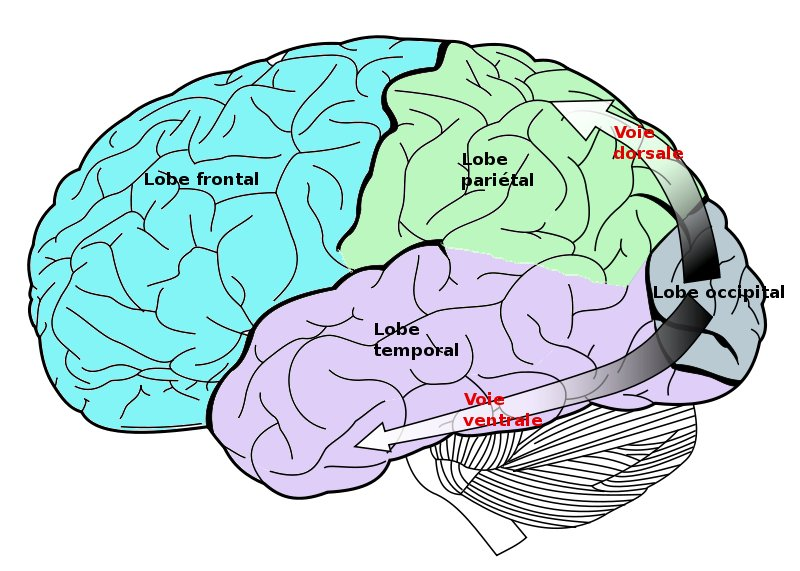
\includegraphics[width=12cm,height=8cm]{figures/ch2_4_Lobes}
\end{center}
\caption{ Les deux voies de traitement visuel. Voie ventrale : reconnaissance, identification des objets. Voie dorsale : traitement des informations, actions [Adapté de wikipedia].}
\label{path}
\end{figure}
%%%%%%%%%

La voie dorsale (appelée aussi la voie du ``comment ?'', \textit{the ``How'' pathway}) commence par \gls{v1}, passe par \gls{v2}, l'aire \gls{mt} puis le cortex pariétal postérieur [\gls{ppc}] \cite{Goodale:1992}. Elle est vouée principalement à guider spatialement les interactions avec les objets du monde visuel. Ce traitement semble être largement inconscient. La voie dorsale est considérée comme une voie d'action car en intégrant les relations spatiales avec notre environnement, ça nous permet d'interagir efficacement avec lui. Cette voie permet le contrôle des mouvements des yeux et des bras surtout quand l'information visuelle est utilisée pour guider des saccades. Nous allons nous intéresser plus à cette voie c'est pourquoi le lobe temporal ne sera pas considéré dans la suite.\\


\subsection{Le lobe pariétal}

Le lobe pariétal participe à l'intégration des informations sensorielles en provenance de différentes parties du corps, la connaissance des membres et de leurs relations, \cite{Blakemore:2005, Fogassi:2005} et  la manipulation d'objets. Certaines parties du lobe pariétal sont impliquées dans le traitement visuo-spatial, plus particulièrement le cortex pariétal postérieur (\gls{ppc}). Bien qu'il soit une zone d'intégration multisensorielle, le cortex pariétal postérieur est désigné comme la voie dorsale de la vision (par opposition à la voie ventrale dans le lobe temporal). \\

Le cortex pariétal du singe est situé en aval du gyrus post-central. Il peut être divisé en deux parties principales: une antérieure et une postérieure. La partie antérieure [\gls{apc}] contient les aires de Brodmann 1, 2, 3 et 43, et le cortex somatosensoriel primaire. La partie postérieure (\gls{ppc}) se compose de aires 5a, 5b, 7a, 7b, et les aires intrapariétales antérieures, latérales, médiales et ventrales (AIP, LIP, MIP et VIP, respectivement).\\

Chez l'homme, le \gls{ppc} peut être subdivisé en lobule pariétal supérieur (aires de Brodmann 5 et 7 correspondant aux aires 5a et 5b chez le singe) et lobule pariétal inférieur (aires de Brodmann 39 et 40 correspondant aux aires 7a et 7b chez le singe), séparés par le sillon intrapariétal [\gls{ips}], lui-même divisé en médial [\gls{mip}], latéral [\gls{lip}], ventral [\gls{vip}] et antérieur [\gls{aip}].\\

Le lobule supérieur semble avoir un rôle essentiellement somatosensoriel \cite{Rizzolatti:1997}. Par contre, le lobule inférieur semble être plus visuel; les neurones de cette région ont la particularité d'être multimodaux, c'est-à-dire qu'ils sont capables de traiter simultanément des stimuli de différentes natures (auditif, visuel, sensorimoteur, etc) \cite{DeRenzi:1982, Rizzolatti:1997}.\\

%%%%%%%%%%%%%%%%%%%%%%%%%Inferior LOBE %%%%%%%%%%%%%%%%%%%%%%%%%%%%%%%%%%%%%%%%%%%%%%%%%

%%%%%%%%%%%%%%%%%%%%%%%%%Intraparietal LOBE %%%%%%%%%%%%%%%%%%%%%%%%%%%%%%%%%%%%%%%%%%%%%%%%%

Enfin, plusieurs études menées dans les années 1990 ont montré que les différentes aires de l'\gls{ips} chez les macaques représentent les différentes parties de l'espace:
\begin{itemize}
\item L'\gls{aip} contient des neurones sensibles à la forme, la taille et l'orientation des objets à saisir \cite{Murata:2000} et à la manipulation des mains \cite{Fogassi:2005}. Il semble être impliqué dans les mouvements de saisie et le codage des objets 3D disposés avant de les saisir.
\item La \gls{mip} contient des neurones qui codent l'emplacement d'une cible en coordonnées  centrées sur le nez \cite{Pesaran:2006}.
\item La \gls{lip} contient une carte rétinotopique \cite{Kusunoki:2003} de neurones  qui représente la saillance des positions spatiales et l'attention à leur accorder. Il permet donc de guider les saccades oculaires \cite{Goldberg:2006}.
\item La \gls{vip} reçoit des projections de plusieurs modalités \cite{Avillac:2005}. Il contient des neurones avec des champs récepteurs tactiles qui codent en coordonnées centrées sur la tête et d'autres avec des champs récepteurs visuels qui codent en coordonnées centrées sur la tête ou les yeux.\\
\end{itemize}

Des études plus récentes ont montré que les humains ont les mêmes régions fonctionnelles dans le sillon intrapariétal \cite{Culham:2006}. En particulier, le champ oculaire pariétal [\gls{pef}], qui correspond à la \gls{lip} chez le singe \cite{Perry:2000}, semble aussi être organisé en coordonnées centrées sur l'oeil de sorte que son activité est mise à jour lorsque les yeux bougent \cite{Medendorp:2003}.\\

De manière plus générale, le \gls{ppc} semble être impliqué dans plusieurs tâches sensori-motrices, et plus particulièrement visuo-motrices:\\
\begin{itemize}
\item[$\bullet$] \textit{L'intégration multi-sensorielle}:
Le \gls{ppc} offre une représentation spatiale multimodale de l'information provenant de différentes modalités sensorielles (vision, audition et somatosensation) avec une copie efférente des mouvements corporels \cite{Andersen:1997}.\\
\item[$\bullet$] \textit{Le contrôle oculomoteur (initiation des saccades)}:
Après des lésions du \gls{pef} chez l'homme (mais pas après une lésion des \glspl{fef} ou des \glspl{sef}), la latence des saccades déclenchées augmente de façon significative \cite{Pierrot:1991}. Le rôle du \gls{pef} dans le processus de déclenchement de saccades (réflexes en particulier) en réponse à des stimuli visuels ou auditifs est discuté dans \cite{Leigh:2004}.\\
\item[$\bullet$] \textit{Le ``remapping'' spatial}:
Des études neurophysiologiques chez des singes montrent que le \gls{ppc} contient plusieurs représentations spatiales\footnote{Ces représentations spatiales peuvent être codées en coordonnées centrées sur le regard, sur les yeux, sur la tête ou centrées sur le corps.} de l'action et soutiennent donc son implication dans la planification des saccades \cite{Colby:1996}. Certains neurones de la \gls{lip} ont en particulier montré des changements dans l'activité neuronale pré-saccadique\footnote{ Un tel comportement n'est pas exclusif à ce champ oculaire, des activités similaires ont été observées dans les \glspl{fef} \cite{Goldberg:1990,Bruce:1985} et dans le colliculus \cite{Mays:1980}.} qui semblent être le signe d'un ``remapping'' spatial qui tient compte des mouvements de l'oeil et du corps \cite{Ross:2001,Duhamel:1992}.\\
\item[$\bullet$] \textit{L'intégration sensori-motrice}:
Il s'agit d'abord de la conversion entre les référentiels associés aux différentes parties du corps qui sont nécessaires pour l'action, car les mouvements des membres peuvent avoir besoin d'être codés dans des coordonnées spatiales différentes de celles utilisées pour la vision. L'emplacement du \gls{ppc} entre les aires visuelles primaires du cortex occipital et le cortex moteur primaire, et ses liens avec les autres aires oculomotrices telles que celles du lobe frontal, le rend idéalement placé pour servir de médiateur des transformations sensori-motrices \cite {Rizzolatti:1997, Machado:2004}. Cette fonction sera traitée avec plus de détails à la fin du chapitre.\\
\item[$\bullet$] \textit{L'attention versus l'intention }:
Plusieurs travaux ont suggéré que le \gls{ppc} est impliqué dans le codage des intentions motrices avec des régions spécialisées selon les types de mouvements \cite{Andersen:2002, Mountcastle:1975}. Contrairement à cela, Colby et Goldberg \cite{Colby:1999} ont proposé que l'activité pariétale reflète plutôt l'attention visuo-spatiale \cite{Bisley:2003}. Le lobe pariétal est supposé contenir des cartes neuronales qui représentent l'emplacement des objets saillants et les actions qui peuvent être effectuées sur eux \cite{Colby:1996}.
L'activité d'une population de neurones dans le \gls{ppc} a été évaluée par \cite{Quiroga:2006} qui ont tenté de prédire l'emplacement de la cible en se basant à la fois sur le lieu de l'attention et le type du mouvement. Comme l'a noté \cite{List:2006}, cette étude est importante pour le débat attention/intention, car si les cellules de la \gls{lip} codent seulement l'attention sur un emplacement alors le type de mouvement à faire ne devrait pas avoir d'effet sur l'activité neuronale. Les résultats suggèrent que l'activité dans le \gls{ppc} peut coder à la fois l'emplacement et l'action, ce qui rejoint la théorie prémotrice (\textit{Premotor theory}) qui porte sur la relation entre l'attention spatiale et la préparation motrice et qui propose que le mécanisme présenté habituellement comme la préparation de l'action motrice (par exemple la préparation d'une saccade oculaire) soit lui-même l'attention \cite{Rizzolatti:1994}.\\


   


\end{itemize}


%%%%%%%%%%%%%%%%%%%%%%%%%%%%%%%%%%%%%%%%%%%%%%%%%%%%%%%%%%%%%%%%%%%%%%%%%%%%%%%%%%%%%%%%%%%%%%%%%%%%%%%%%%%%%%%%%%%%%%%%%%%%%%%%%%%%%%%%%%%%%%%%%%%%%%%%%%%%%%%%%%%%%%%%%%%%%%%%%%%%%%%%%%%%%%%%%%%%%
%%%%%%%%%%%%%%%%%%%%%%%%%%%%%%%%%%%%%%%%%%%%%%%%%%%%%%%%%%%%%%%%%%%%%%%%%%%%%%%%%%%%%%%%%%%%%%%%%%%%%%%%%%%%%%%%%%%%%%%%%%%%%%%%%%%%%%%%%%%%%%%%%%%%%%%%%%%%%%%%%%%%%%%%%%%%%%%%%%%%%%%%%%%%%%%%%%%%%

\subsection{Le lobe frontal}

Le cortex frontal des primates comprend deux principales zones identifiées pour le contrôle des mouvements des yeux \cite{Schall:1997, Tehovnik:2000}: les champs oculaires frontaux [\glspl{fef}] et les champs oculaires supplémentaires [\glspl{sef}] (fig \ref{struct}).\\

\begin{figure}
\begin{center}
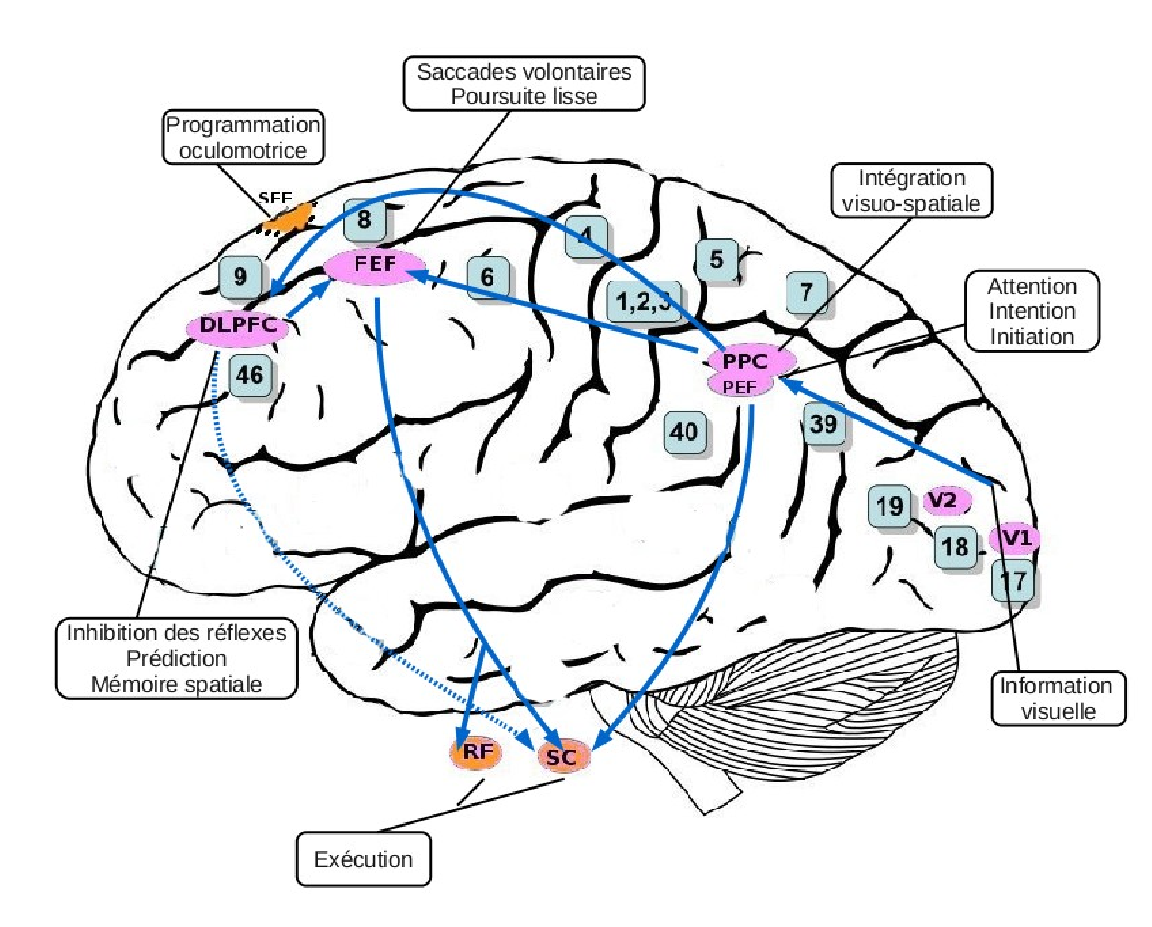
\includegraphics[width=14cm,height=10cm]{figures/ch2_5_Structures}
\end{center}
\caption{Quelques structures impliquées dans la génération des saccades. Après avoir reçu l'information visuelle dans le lobe occipital et après l'intégration visuo-spatiale dans PPC, une saccade peut être déclenchée soit par réflexe, principalement par PEF, ou intentionnellement par FEF, une zone qui semble également être impliquée dans la fixation visuelle active. Si une saccade réflexe doit être inhibée, DLPFC semble y participer. Cette zone est également impliquée dans la mémoire spatiale à court terme et la prédiction. Avec ces trois actions différentes, DLPFC assure un rôle important dans les processus décisionnels de contrôle du comportement moteur oculaire. SEF pourrait être impliqué dans les contrôles de haut niveau tels que les transformations spatiales, les mouvements appris et l'ajustement des programmes moteurs. SC code l'amplitude et la direction des saccades volontaires. FEF et SC projettent sur RF qui contient les centres vertical et horizontal du regard. RF envoie les commandes de déclenchement de saccades vers les neurones moteurs qui innervent les muscles extraoculaires. DLPFC = cortex préfrontal dorsolatéral; FEF = champ oculaire frontal; PEF = champ oculaire pariétal; PPC = cortex pariétal postérieur; RF= formation réticulée ; SC = colliculus supérieur; SEF = champ oculaire supplémentaire; Le trait discontinu correspond à l'inhibition des saccades. Les zones numérotées correspondent aux aires de Brodmann. [adapté de wikipedia]}

\label{struct}
\end{figure}
%http://brain.oxfordjournals.org/content/126/6/1460/F6.expansion
\subsubsection{Les champs oculaires frontaux}
%%%%%%%%%%%%%%%%%%%%%%%%%%%%%%%%%%%%%%%%%%%%%%%%%%%%%%%%%
Les \glspl{fef} sont situés dans le cortex préfrontal le long de la convexité latérale supérieure correspondant globalement à l'aire de Brodmann 8 et des parties des aires 9 et 6 \cite{Bruce:1985} (fig \ref{struct}). L'implication des \glspl{fef} dans le contrôle oculomoteur a été montrée par la stimulation de Ferrier de l'aire corticale 8 prémotrice chez les singes qui a provoqué des mouvements oculaires contralatéraux \cite{Ferrier:1874}. En effet, les \glspl{fef} forment une structure topographique et représentent les cibles des saccades dans des coordonnées rétinotopiques \cite{Bruce:1985}. Leur stimulation chez le singe rhésus suscite des mouvements des yeux vers une direction spécifique ainsi que la dilatation pupillaire. Chez l'homme l'activation des \glspl{fef} pendant les saccades a été démontrée par les travaux de \cite{Melamed:1979, Petit:1993}.\\

Les cellules des \glspl{fef} s'activent en réponse sélective à des stimuli visuels fixes ou mobiles à portée des bras, ainsi qu'à des stimuli tactiles et auditifs \cite{Rizzolatti:1981}. Ces cellules sont fortement impliquées dans la médiation de l'attention visuelle et la coordination des réactions de la tête, des bras et des yeux \cite{Denny:1966, Gottlieb:1994, Macavoy:1991, Pragay:1987, Segraves:1987, Wagman:1961}. Les \glspl{fef} permettent en particulier de guider le regard dans le choix des cibles en transformant l'information visuelle en une réponse d'orientation \cite {Schall:2002, Schall:2004, Wurtz:1980, Segraves:1987} (certaines cellules signalent l'emplacement des stimuli bien visibles et significatifs qui peuvent être des cibles pour les saccades volontaires) et de contrôler si et quand une saccade vers une cible donnée est déclenchée. Des lésions des \glspl{fef} peuvent donc altérer la capacité de réaliser des saccades volontaires ou augmenter leurs latences \cite{Stuphorn:2002, Macavoy:1991, Schall:2002}.\\

Les \glspl{fef} sont aussi impliqués dans des mouvements de poursuite lente \cite{Gottlieb:1994} et le guidage des mouvements lors de la lecture et l'écriture \cite{Ritaccio:1992}. Enfin, l'activité des neurones dans les \glspl{fef} met en évidence un rôle d'anticipation \cite{Gottlieb:1994, Pragay:1987}. En fait, certains neurones s'activent avant qu'une réponse des yeux ne soit déclenchée et continuent à tirer à une cadence élevée jusqu'à ce que le comportement soit lancé. \\




%%http://brainmind.com/FrontalEyeFieldsArea8.html

\subsubsection{Les champs oculaires supplémentaires}

La région des \glspl{sef} a d'abord été décrite chez les primates non humains. Elle occupe la partie la plus rostrale du cortex prémoteur dorsal appelée l'aire F7 \cite{Matelli:1991}. Elle projette vers des structures corticales et sous-corticales incluses dans la génération de saccades \cite{Huerta:1990, Parthasarathy:1992, Schall:1993, Shook:1990}. Ces connexions sont plus diffuses que celles des \glspl{fef}. L'organisation fonctionnelle des \glspl{sef} a été étudiée par l'analyse de l'activité pré-saccadique et la stimulation électrique. Ils ont été d'abord caractérisés par John Schlag et ses collègues comme une zone où la stimulation électrique de faible intensité peut évoquer des saccades \cite{Schlag:1987}. Puis il a été montré que la stimulation des \glspl{sef} produit des mouvements coordonnés des yeux et de la tête \cite{Martinez:2003} d'o\`u l'hypothèse que les \glspl{sef} encodent les mouvements saccadiques centrés sur la tête et non pas sur l'oeil (en coordonnés rétiniennes).\\

En effet, les neurones dans les \glspl{sef} réagissent à des stimuli visuels et acoustiques et sont actifs avant et pendant les mouvements oculaires \cite{Berdyyeva:2009, Bon:1991, Ohmae:2008, Schlag:1992,Nakamura:2005, Uchida:2007} participant en particulier à la planification, l'exécution et le contrôle  des saccades volontaires, réflexes et les mouvements de poursuite lente.\\ 

%, Hanes et al 1995;. Heinen, 1995; Lee et Tehovnik 1995; Moorman et Olson, 2007a, b; Nakamura et al 2005;. Ohmae et al 2008;. Pouget et al 2005, S
Les similitudes anatomiques et physiologiques entre les \glspl{sef} et les \glspl{fef} ont conduit à l'hypothèse qu'ils agissent en parallèle \cite{Amador:2004, Russo:2000, Tehovnik:2000}. Cependant, de nombreuses caractéristiques les distinguent. Les saccades évoquées par la microstimulation des \glspl{fef} sont généralement vectorielles: les yeux se déplacent de la même distance dans le même sens quelle que soit la position initiale. En revanche, celles évoquées par la microstimulation des \glspl{sef} ont tendance à être orientées but (convergentes): en partant de différentes positions initiales, les yeux arrivent à une seule position finale \cite{Martinez:2004, Park:2006}.\\
%, Russo et Bruce 1993; Schall 1991; Schlag et Schlag-Rey, 1987; Tehovnik et Lee, 1993

Les \glspl{sef} présentent en plus des profils d'activité neuronale pré-saccadique nettement différents de ceux enregistrés dans les \glspl{fef} et qui semblent en plus dépendre du contexte \cite{Amador:2004, Chen:1995, Isoda:2002,  Ohmae:2008, Uchida:2007}.
%Coe et al 2002, 2003; Lu et al . 2002;. Mushiake et al 1996; Nakamura et al 2005,Olson et Gettner 1995, 1999; Schlag-Rey et al 1997;. Tremblay et al 2002, 
L'activation neuronale dans les \glspl{sef} est en particulier corrélée avec le temps de déclenchement de la saccade et permet une prédiction partielle de l'erreur et la probabilité d'annulation \cite{Nakamura:2005, Amador:2000, Roesch:2003, Stuphorn:2000}.\\

Il en résulte que le rôle des \glspl{sef} dans le contrôle du comportement oculomoteur ne se réduit pas à l'initiation de saccades. Cette région s'avère être impliquée dans des aspects de haut niveau de contrôle de mouvements oculaires comme les transformations spatiales complexes \cite{Olson:1995}, les mouvements appris\cite{Chen:1995}, les fonctions cognitives exécutives \cite{Stuphorn:2006} et contribue à l'ajustement dynamique de la génération de saccades \cite{Stuphorn:2010}.\\

\subsubsection{Le cortex pr\'efrontal dorsolat\'eral}
%%%http://brain.oxfordjournals.org/content/127/3/460.full
Une autre région située sur la surface dorsolatérale du lobe frontal, participe au contrôle des saccades volontaires: le cortex préfrontal dorsolatéral [\gls{dlpfc}]. Elle correspond aux aires de Brodmann 46 et 9 situées dans le gyrus frontal moyen et le cortex adjacent (fig \ref{struct}). Le \gls{dlpfc} diffère des autres champs oculomoteurs par le fait que sa stimulation ne déclenche pas de saccades.\\

Les patients atteints de lésions du \gls{dlpfc} ont des difficultés à inhiber les saccades réflexes. Dans la tâche anti-saccade, ces lésions provoquent une augmentation du pourcentage d'erreurs due à l'affaiblissement des facultés d'inhibition de mouvements oculaires réflexes \cite{Pierrot:2003}. En revanche, les patients atteints de lésions des \glspl{fef} ont un pourcentage normal d'erreurs sur la même tâche mais leurs anti-saccades correctes s'effectuent avec un temps de latence plus long que chez les sujets normaux. Ainsi, il a été supposé qu'au cours de la tâche anti-saccade, l'inhibition de saccades réflexes mal acheminées est due au \gls{dlpfc}, alors que le déclenchement intentionnel des antisaccades correctes dépend des \glspl{fef} \cite{Rivaud:1994, Pierrot:2003}.\\

Le \gls{dlpfc} est supposé aussi être impliqué dans la mémorisation à court terme (jusqu'à 20 secondes) de l'information visuo-spatiale importante (position d'une cible par exemple). En effet, l'activité des neurones du \gls{dlpfc} chez le singe, lors des tests de saccades guidées par des cibles mémorisées, montre la présence d'une carte mémoire topographique \cite{Sawaguchi:2001}. Chez l'homme, on remarque aussi une activation du \gls{dlpfc} lors de l'exécution de la même tâche \cite{Sweeney:1996}. De plus, lorsque le \gls{dlpfc} chez le singe est inactivé pharmacologiquement, les saccades guidées par la mémoire sont altérées et le pourcentage d'erreurs augmente \cite{Sawaguchi:1994}, de même pour les sujets humains qui sont atteints de lésions du \gls{dlpfc} \cite{Pierrot:2003} .\\

Enfin dans ces derniers cas, les saccades prédictives sont également altérées. Le \gls{dlpfc} semble également être la structure la plus impliquée quand une réponse est prédite à un emplacement spécifique (avant l'apparition du stimulus). Vraisemblablement, la mémoire de travail est nécessaire pour générer des réponses prédictives \cite{Pierrot:2003}.\\

Ces résultats suggèrent que le \gls{dlpfc} joue un rôle crucial dans les processus décisionnels, la préparation de saccades en inhibant les saccades réflexes indésirables (processus d'inhibition intentionnelle), le maintien  de l'information en mémoire pour des saccades volontaires (processus de mémorisation spatiale à court terme) et la facilitation des saccades anticipatrices (processus de prédiction), en fonction des circonstances environnementales.\cite{Pierrot:2003, Leigh:2006}.\\



%%%%%%%%%%%%%%%%%%%%%%%%%%%%%%%%%%%%%%%%%%%%%%%%%%%%%%%%%%%%%%%%%%%%%%%%%%%%%%%%%%%%%%%%%%%%%%%%%%%%%%%%%%%%%%%%%%%%%%%%%%%%%%%%%%%%%%%%%%%%%%%%%%%%%%%%%%%%%%%%%%%%%%%%%%%%%%%%%%%%%%%%%%%%%%%%%%%%%
%%%%%%%%%%%%%%%%%%%%%%%%%%%%%%%%%%%%%%%%%%%%%%%%%%%%%%%%%%%%%%%%%%%%%%%%%%%%%%%%%%%%%%%%%%%%%%%%%%%%%%%%%%%%%%%%%%%%%%%%%%%%%%%%%%%%%%%%%%%%%%%%%%%%%%%%%%%%%%%%%%%%%%%%%%%%%%%%%%%%%%%%%%%%%%%%%%%%%





\subsection{Le colliculus supérieur}




Le colliculus supérieur [\gls{sc}] est une structure sous corticale qui se trouve sur le tectum du mésencéphale. Cette structure est directement impliquée dans le mécanisme de génération et de contrôle des saccades \cite{Nolte:1993,Ziad:1999}. Il existe deux colliculi supérieurs, un dans chaque hémisphère du cerveau (symétrie bilatérale du cerveau).\\


Le \gls{sc} sert de site d'intégration sensori-motrice qui reçoit des entrées somato-sensorielles, auditives et visuelles \cite {Nolte:1993}. Ses entrées visuelles proviennent soit directement de la rétine ou soint indirectement en passant par le cortex (modulé par l'intervention d'autres structures). L'intégration permet de transformer les entrées sensorielles portant sur la position du stimulus pour fournir les ordres ou les prédictions de déplacements à des muscles extra-oculaires par l'intermédiaire des neurones moteurs \cite {Wurtz:1996, Nolte:1993}.\\

Une caractéristique clé du \gls{sc} est son organisation en couches. La couche superficielle est une couche visuelle qui reçoit des informations directement des cellules ganglionnaires de la rétine. Chaque site de cette couche est activé par un stimulus optimal présent dans une position particulière dans le champ visuel. Cependant, la couche profonde constitue une carte motrice organisée topographiquement: les vecteurs saccades résultant d'un stimulus visuel dépendent de la position du stimulus.\\


De nombreux modèles ont étudié le rôle du \gls{sc} (cf. \cite {Girard:2005} pour une revue). \cite{Findlay:1999} soulignent que sa principale fonction est de décider quand et où la saccade doit être effectuée. Plus tard, \cite {Godijn:2002} ont proposé un modèle d'intégration compétitive fondé sur de solides preuves expérimentales au niveau comportemental, qui indique que toutes les informations (exogènes versus endogènes, spatiales versus traitement temporel) peuvent être intégrées dans une seule carte motrice considérée comme un modèle du \gls{sc}. Plus de données sur cette structure et sur son implication dans la génération des saccades seront détaillées dans le chapitre 3 qui portera sur la proposition d'un modèle du \gls{sc}.\\

\subsection{Les ganglions de la base}

Les noyaux gris centraux (appelés encore les ganglions de la base) [\gls{bg}] sont un ensemble de noyaux situés des deux côtés du thalamus, en dehors et au-dessus du système limbique. Plusieurs études suggèrent que les \gls{bg} participent à la régulation de l'activité corticale par un mécanisme de désinhibition (retrait de l'inhibition) de l'activité thalamique considéré comme struture de centralisation des informations sensorielles et motrices. Ces noyaux assurent un ensemble d'intégration dans des circuits distincts fonctionnellement. En particuler, ces noyaux participent à la modulation de l'activité colliculaire via le circuit oculomoteur. \\

De manière schématique, les \gls{bg} agissent de deux manières sur les mouvements oculaires. D'abord, ils facilitent l'initiation des saccades volontaires générées dans un contexte de comportements appris, de prédiction ou de récompense retardée. Cette facilitation est réalisée par la désinhibition des couches intermédiaires du \gls{sc} qui sont sous inhibition tonique (empêchant le déclenchement de saccades). Le colliculus supérieur est alors ``libéré'' et la génération de saccades est rendue possible. Ensuite, ils permettent d'empêcher la génération de saccades réflexes non souhaitées \cite{Leigh:2006}. Une description plus détaillée de cette structure sera donnée dans le chapitre 4 en abordant, en particulier, son rôle dans la sélection de l'action.\\

\subsection{La formation réticulée}


La formation réticulée [\gls{rf}] est une structure nerveuse du tronc cérébral. De manière générale, elle permet la coordination et la synthèse des actions. Le système réticulé intervient dans la régulation de grandes fonctions vitales telle que la respiration et les cycles éveil-sommeil, la motricité en général et dans des fonctions cognitives telles que l'attention. Elle reçoit des entrées de pratiquement tout le cerveau. La \gls{rf} est en particulier chargée de générer les saccades oculaires permettant d'amener le centre d'intérêt sur la fovéa.\\

La direction des mouvements oculaires est pilotée par deux centres de la \gls{rf} (deux générateurs saccadiques):
\begin{itemize}
\item les mouvements horizontaux par la formation réticulée pontique paramédiane [\gls{pprf}] qui se trouve dans la région caudale du tronc cérébral, le long de la ligne médiane (centre horizontal du regard).
\item les mouvements verticaux par la formation réticulée mésencéphalique [\gls{mrf}] (centre vertical du regard). 
\item les mouvements obliques proviennent de leur action conjointe.\\
 \end{itemize}

\begin{figure}
\begin{center}
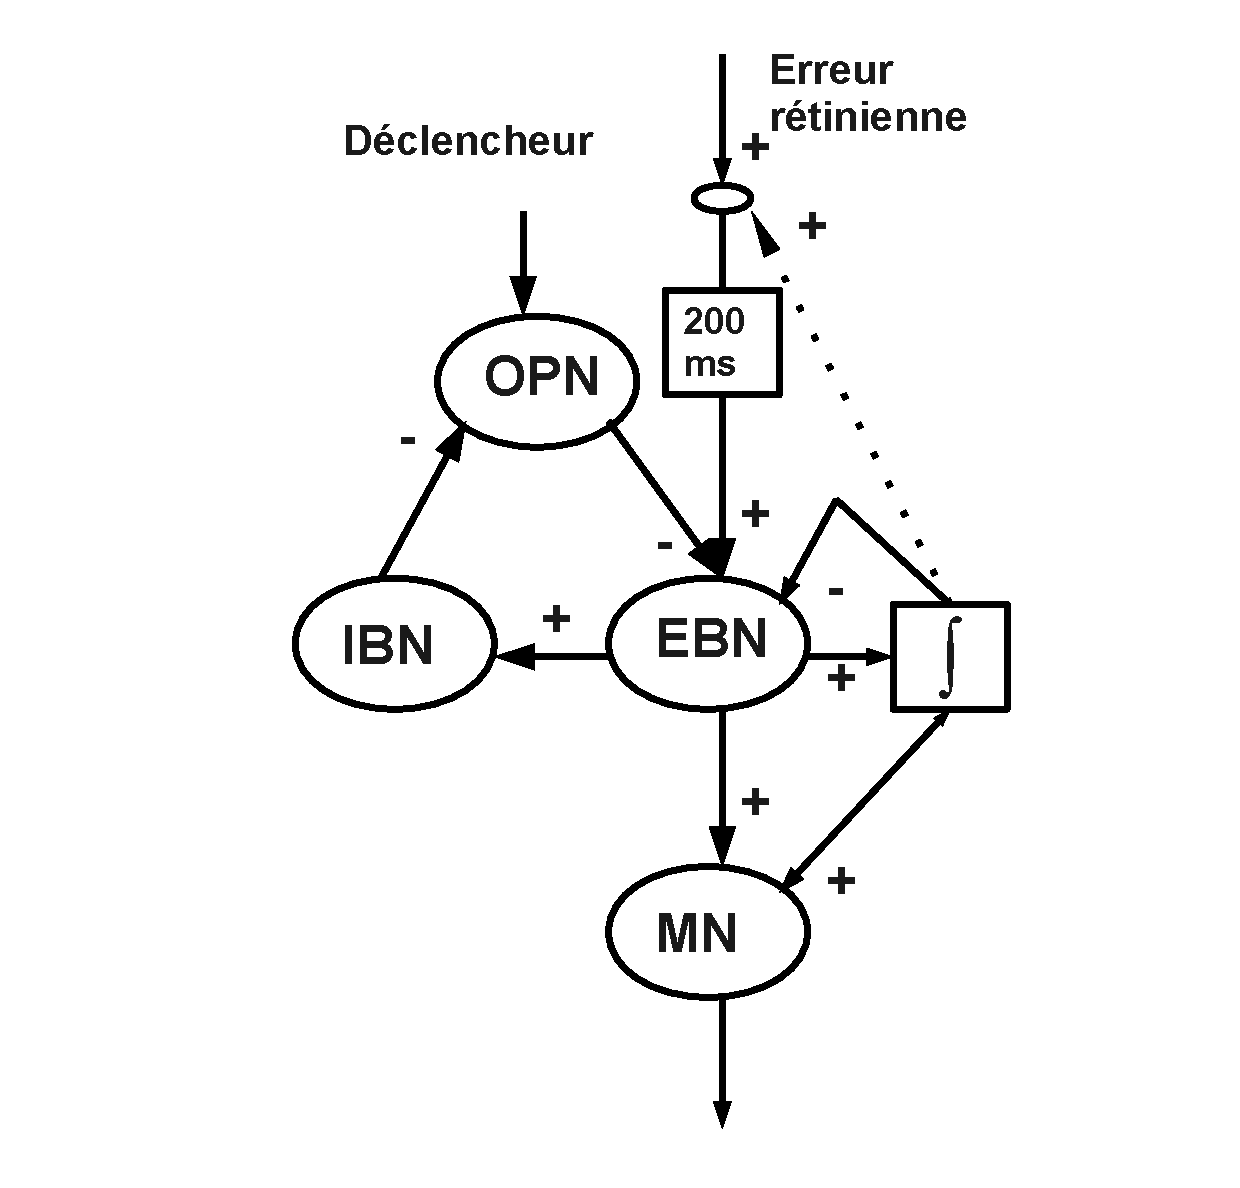
\includegraphics[width=0.5\textwidth]{figures/ch2_6_Robinson}
\end{center}
\caption{Le modèle original du générateur saccadique proposé par \cite{Robinson:1975} avec un seul intégrateur et un feedback local. Les (+) désignent les projections excitatrices et les (-) désignent les projections inhibtrices}
\label{robinson}
\end{figure}

Plusieurs types de neurones de la \gls{rf} assurent une fonction prémotrice de générateurs saccadiques \cite{Scudder:2002} en projettant vers les motoneurones [\gls{mn}] du tronc cérébral commandant les muscles oculaires. L'activité tonique des \gls{mn} est assuré par des neurones toniques [\gls{tn}]. Les \gls{tn} et les \gls{mn} qui innervent directement le muscle droit externe ipsilatéral reçoivent des projections des neurones phasiques excitateurs [\gls{ebn}] pendant les saccades ipsilatérales. Des neurones phasiques inhibiteurs [\gls{ibn}] s'activent, eux aussi, pendant les saccades ipsilatérales et projettent vers les \gls{mn} contralatéraux et les \gls{tn}. Par contre, des neurones omnipauseurs [\gls{opn}] s'activent pendant les phases de fixation et sont inactifs pendant les saccades. Ils inhibent les neurones phasiques à latence moyenne [\gls{mlbn}] qui s'activent avant le déclenchement d'une saccade. Enfin, des neurones phasiques à longue latence [\gls{llbn}] déchargent à leur fréquence maximale au moment de déclenchement de la saccade. Les interactions entre ces différentes classes de neurones ont été étudiées dans plusieurs modèles de générateurs saccadiques \cite{Robinson:1975,Tweed:1985,Scudder:1988,Quaia:1997} (voir par exemple la figure \ref{robinson}).






\subsection{Le cervelet}
%%%%%%%%%%%%%%%%%%%%%%%%%%%%%%%%%%%%%%%%%%
Le cervelet est une structure de l'encéphale des vertébrés située dans la fosse crânienne postérieure. Le cervelet est considéré comme l'organe de régulation motrice qui coordonne et module les mouvements. L'une de ses fonctions principales est d'évaluer et de rectifier l'exécution des mouvements déclenchés par les aires motrices du cortex cérébral. Deux sous-divisions du cervelet jouent des rôles importants dans le contrôle des mouvements oculaires volontaires \cite{Noda:1987,Robinson:2001}.\\ %\cite {hitzig et ferrier (simulation electrique), holmes et cogar (cliniquement)}.\\
 
%Le vermis dorsal cérébelleux (lobules VI et VII) et la partie caudale du noyau fastigial (Noda et Fujikado, 1987; Robinson et Fuchs, 2001).
D'abord, le cervelet vestibulaire est impliqué dans les interactions vestibulo-visuelles et dans la stabilisation du regard. Il peut s'agir de stabiliser les yeux sur une cible fixe ou sur une cible en mouvement pour une poursuite lente. Dans le cas du réflexe vestibulo-oculaire, il peut aussi s'agir de stabiliser le regard malgré des mouvements perturbateurs de la tête.\\

Ensuite le vermis dorsal cérébelleux (lobules VI et VII) et la partie caudale du noyau fastigial contrôlent principalement la précision des saccades.
Certains neurones du vermis dorsal encodent avec précision le moment où une saccade doit s'arrêter pour atteindre une cible prévue. Ce contrôle de la précision est assuré par les ``feed-back'' continus que reçoit le cervelet (informations sur la position et la vitesse de l'oeil, la position et la vitesse de la cible et les commandes motrices \cite{Leigh:2006, Fuchs:1993}. \\

%%%%%%%%%%%%%%%%%%%%%%%%%%%%%%%%%%%%%%%%%%%%%%%%%%%%%%%%%%%%%%%%%%%%%%%%%%%%%%%%%%%%%%%%%%%%%%%%%%%%%%%%%%%%%%%%%%%%%%%%%%%%%%%%%%%%%%%%%%%%%%%%%%%%%%%%%%%

\subsection{Le thalamus}

Le thalamus [\gls{th}] est une structure symétrique située entre le cortex cérébral et le mésencéphale. Il est considéré comme un point relai entre les différentes structures corticales et sous-corticales qui permet de centraliser l'information sensorielle et motrice. Pour le système visuel, par exemple, les entrées de la rétine sont envoyées vers le \gls{lgn} du thalamus (voir \cite{Guillery:2002} pour une revue).\\

John LeDoux \cite{Ledoux:1998} a mis en évidence le rôle du \gls{th} dans l'analyse et le traitement des informations. Il ne s'agit pas donc seulement d'un point relai. LeDoux a mis en évidence deux circuits: le premier analyse rapidement l'image dans une forme générale floue et détecte les situations d'urgence pour activer les réactions émotionnelles avant que l'information n'arrive au cortex. En parallèle, les influx nerveux continuent leur chemin vers le cortex qui analyse beaucoup plus finement, module et nuance la perception et modifie les émotions. Un exemple classique est celui d'un objet ayant une forme allongée vu sur le sol, le thalamus l'interprète comme un serpent et active les réactions corporelles et émotionnelles. Le cortex peut ensuite analyser plus finement et réaliser que ce n'était qu'un tuyau d'arrosage et limiter ou moduler l'action de l'amygdale.\\

Des expériences sur les animaux montrent qu'au moins deux parties du thalamus participent à la programmation des saccades: la lame médullaire interne [\gls{iml}] et le thalamus pulvinaire [\gls{pt}] \cite{Schlag:1984,Robinson:1986}. L'\gls{iml} reçoit des entrées de structures corticales et du tronc cérébral concernées par les mouvements oculaires mais projette seulement vers le cortex et les ganglions de la base. Il pourrait être une source de copies efférentes pour les aires corticales. La présence d'activations des neurones de l'\gls{iml} liées à des mouvements oculaires est compatible avec son implication dans le contrôle des saccades visuellement guidées \cite{Schlag:1989}. Le \gls{pt}, situé dans la partie postérieure du thalamus, participe à la gestion des conséquences visuelles des mouvements oculaires. Il participe aussi à la boucle basalo-colliculaire sous-corticale \cite{McHaffie:2005}. Il envoie des projections vers \gls{mt}. Il projette aussi sur le lobe pariétal et pourrait contribuer au déplacement de l'attention visuelle \cite{Benevento:1995, Olshausen:1993}.\\





Enfin, en examinant les projections et les connexions entre les différentes structures et aires décrites précédemment, nous constatons que le traitement de l'information visuelle peut suivre plusieurs voies rapides ou lentes selon les interactions mises en oeuvre. La complexité du traitement dépend donc des voies empruntées mais une problématique commune à toutes les voies concerne la transformation de l'information visuelle en information motrice.\\

\section{Contr\^ole nerveux des saccades: transformation visuo-motrice}

Les saccades oculaires peuvent survenir dans l'obscurité mais elle sont souvent déclenchées quand quelque chose attire l'attention (visuellement, auditivement...). Comment les informations sensorielles relatives à la position spatiale de la cible sont elles transformées en un pattern adéquat d'activités de neurones de centres de contrôles horizontal et vertical responsables des réactions motrices?\\

Deux structures projettent principalement sur ces centres moteurs: Le \gls{sc} et les \glspl{fef} (fig \ref{struct}). Les deux ont des neurones moteurs qui déchargent juste avant les saccades et contiennent une représentation topographique. Ces deux structures pré-motrices comportent des neurones qui répondent aux stimuli visuels mais les relations entre les réponses sensorielles et motrices ont été plus étudiées dans le \gls{sc} \cite{Lefevre:1998, Quaia:1999}. Les neurones d'une région précise du \gls{sc} s'activent par la présence d'un stimulus visuel dans une région restreinte de l'espace visuel: cette activation provoque une saccade déplaçant l'oeil d'une distance précise \cite{Schiller:1972}. En outre, La stimulation électrique du \gls{sc} profond chez l'animal à tête fixe évoque des déplacements du regard avec des directions fixes dans les coordonnées oculocentrées mais qui varient en fonction de la position initiale \cite{Klier:2001}. La carte motrice du \gls{sc} encode donc spatialement les coordonnées (amplitude et direction) des saccades à venir en coordonnées rétiniennes \cite{Hepp:1993, VanOpstal:1991}.\\



Par contre, la représentation neuronale des commandes motrices est différente, les neurones oculomoteurs encodent les caractéristiques de la saccade en fonction de l'activation des neurones moteurs et non pas de leurs positions. L'information visuelle codée par les neurones sensoriels et pré-moteurs doit être transmise aux neurones moteurs et convertie en commandes motrices. Il s'agit d'une transformation visuo-motrice. Le cerveau transforme donc le stimulus qui est codé sous forme de position de neurones actifs (\textit{codage spatial}) en une commande motrice sous forme de fréquence et durée de décharge (\textit{codage temporel}) \cite{Moschovakis:1994, Robinson:1968, Sparks:1990, Sparks:2002}.\\

En effet, l'image de l'objet est d'abord captée par la rétine. Sa représentation est donc d'abord codée dans un référentiel rétinocentré. La transformation visuo-motrice commence par spécifier la différence vectorielle entre le point de regard courant et le point de regard souhaité doit être spécifiée (erreur rétinienne spatiale) et se termine par une commande motrice servant à bouger les yeux vers l'endroit désiré (erreur motrice temporelle) \cite{Robinson:1968,Tweed:1990, Crawford:1997}. La voie dorsale a pour fonction principale d'extraire, dans le but de guider l'action, des informations spatiales et temporelles (la taille des objets, leur localisation, leur orientation, la direction et la vitesse des mouvements, etc...). Cette voie assurerait donc un rôle essentiel dans les transformations visuo-motrices par l'intermédiaire de circuits pariéto-frontaux.\\



En outre, les saccades évoquées visuellement ont des caractéristiques stéréotypées: leurs trajectoires sont pratiquement droites, il y a une relation constante linéaire entre la durée et l'amplitude du mouvement, le temps d'accélération est presque constant pour toutes les saccades. Les circuits qui codent les commandes motrices pour les saccades doivent également assurer la transformation spatio-temporelle. Les métriques des saccades sont données par une activation spatiale sur une carte topographique, alors qu'il faut fournir une commande sous forme de taux de décharge dans le système de coordonnées adapté aux muscles extraoculaires \cite{Becker:1973, Westheimer:1973}. Un certain nombre de recherches théoriques et physiologiques ont examiné ce problème (par exemple \cite{Hepp:1983, Optican:2002,Tweed:1990}). Cependant, il semble que la transformation physiologique d'un code topographique en une représentation vectorielle pour les deux centres de regard est inséparable de la transformation du référenciel oculomoteur. \\

Enfin, un point de discussion qui est toujours ouvert porte sur comment décoder l'activation de la population de neurones de la couche motrice du \gls{sc}. En particulier, si cette activité porte aussi des informations concernant la trajectoire des mouvements oculaires et sa cinématique (un rôle moteur du \gls{sc}) ou bien si elle encode principalement le vecteur saccade (le \gls{sc} encode le but). C'est cette dernière hypothèse que nous allons adopter dans le chapitre suivant qui portera sur un modèle d'initiation de saccades. \\

En effet, plusieurs schémas de calcul ont été proposés comme mécanismes potentiels pour décoder l'activité colliculaire évoquant une saccade visuelle (voir \cite{Gandhi:2011} pour une revue récente): le vecteur somme \cite{Badler:2002, VanGisbergen:1987}, le vecteur moyenne \cite{Lee:1988, Walton:2005} et le vecteur somme dynamique (ou somme avec saturation) \cite{Goossens:2006,Groh:2001}.\\

Le décodage par vecteur moyenne est calculé en prenant la moyenne pondérée des contributions de chaque neurone de la population active \cite{Lee:1988, Walton:2005}. Ce schéma de calcul permet de rendre compte des résultats de microstimulations simultanées de deux positions dans le colliculus supérieur \cite{Katnani:2010, Robinson:1972}. En effet, l'amplitude et la direction de la saccade résultante sont prédites par la moyenne pondérée des deux saccades générées lorsque chaque position est stimulée séparément. En outre, l'inactivation locale de la carte motrice colliculaire génère des saccades altérées qui correspondent aux prédictions de l'hypothèse de la moyenne \cite{Lee:1988}.\\

Cependant, ce schéma de décodage ne tient pas compte de la relation observée entre le niveau d'activité colliculaire et la vitesse des saccades \cite{Goossens:2000} ou de la diminution de l'amplitude des saccades avec l'intensité de la microstimulation \cite{Groh:2011,Katnani:2010}. Une autre limitation de ce modèle est la difficulté de la mise en oeuvre (physiologiquement) du facteur de normalisation \cite{Groh:2001}.\\

En revanche, le modèle du vecteur somme présente un mécanisme simple et intuitif pour expliquer le décodage des saccades. Dans ce schéma de décodage, il est supposé que chaque neurone colliculaire actif contribue par un vecteur de déplacement qui est pondéré par le taux de décharge moyen de la cellule et que la forme spatiale de l'activation de la carte colliculaire est stéréotypée. La somme résultante de ces vecteurs pondérés produit le déplacement désiré \cite{VanGisbergen:1987}. Ce modèle de somme simple ne permet pas de simuler correctement la stimulation simultanée de deux sites du colliculus ou l'inhibition locale de la carte colliculaire motrice. Ses lacunes peuvent être rattrapées par l'intégration de la connectivité intracolliculaire telles que l'excitation locale et l'inhibition globale \cite{VanOpstal:1989}.\\ 

Les premières versions de ces deux modèles se basent sur l'activité colliculaire statique et ne rendent pas compte des caractéristiques dynamiques de la saccade. Cependant, plusieurs preuves suggèrent que le niveau d'activité colliculaire influence la cinématique des saccades d'o\`u les modèles de décodage dynamique par vecteur somme \cite{Goossens:2006,VanOpstal:2008}. La somme des spikes est limitée par un seuil de saturation \cite{Goossens:2006, Groh:2001}. Une saccade est calculée par la somme vectorielle de toutes les contributions de cellules individuelles à travers le temps. Ainsi, le nombre cumulé de spikes dans la population active est lié au déplacement des yeux en cours. Les simulations du vecteur somme dynamique ont montré plusieurs propriétés des saccades comme la non-linéarité cinématique que les autres modèles ne peuvent pas expliquer sans hypothèses supplémentaires telles que la normalisation de l'activité.\\

Bien que ce mécanisme dynamique révèle des propriétés avantageuses, le calcul donnera toujours une somme vectorielle lorsqu'il est testé avec la contribution simultanée de deux sites actifs. En conséquence, le modèle prédit une addition linéaire à des faibles niveaux d'activité lorsque le seuil n'est pas atteint, mais cette prédiction n'a pas été confirmée par les données de \cite{Katnani:2012} qui proposent donc que les interactions excitatrices et inhibitrices dans la carte colliculaire motrice sont essentielles pour limiter un mécanisme de sommation.\\

Les prédictions de ces différents schémas de décodage ont sollicité de nombreuses expériences qui tentent de valider leurs hypothèses et révéler des propriétés émergentes. Différentes méthodes sont nécessaires pour mieux les différencier à travers les expériences de microstimulation qui exploitent l'influence de la variation des paramètres de stimulation sur les caractéristiques des saccades  \cite{Brecht:2004, Katnani:2010, Katnani:2012}.\\

En résumé, deux modèles courants de décodage de l'activité colliculaire motrice coexistent: vecteur moyenne et vecteur somme. Les premières versions de ces modèles décodent seulement les métriques des saccades. Ensuite, les deux modèles ont été adaptés pour tenir compte de la cinématique. En particulier, un schéma de calcul par sommation dynamique propose que la sortie colliculaire code la trajectoire désirée et la vitesse \cite{Goossens:2006, Groh:2001}. L'évolution de chaque schéma de calcul a montré des avantages et des inconvénients \cite{Gandhi:2011,Katnani:2012} et les travaux récents examinent le dernier schéma de calcul basé sur la sommation dynamique avec saturation. Cependant, ce schéma ne sera pas décrit dans le chapitre suivant car nous nous sommes intéressés au décodage de l'activité colliculaire statique et l'encodage de la position de la cible sans la mise en oeuvre de la saccade et sa dynamique.\\
 








 

%%%%%%%%%%%%%%%%%%%%%%%%%%%%%%%%%%%%%%%%%%%%%%%%%%%%%%%%%%%%%%%%%%%%%%%%%%%%%%%%%%%%%%%%%%%%

\section{Conclusion}


Dans ce chapitre nous avons d'abord passé en revue les mouvements oculaires observés chez les primates pour mieux situer les saccades oculaires par rapport aux autres mouvements, puisque nous allons nous intéresser dans la suite à un modèle d'initiation des saccades en étudiant le flux visuel partant de la rétine vers les couches profondes du colliculus supérieur. En effet, le cadre sous lequel nous voyons le monde est modifié de manière continue par les saccades. En examinant les différents types de saccades listés, la vision n'apparait pas comme simplement le résultat de la perception passive d'un stimulus ou d'une forme mais le résultat de l' ``action de voir'' pour agir sur l'environnement.\\




La mobilité et la coordination des deux yeux (la tête et le reste du corps) sont donc indispensables à l'accomplissement d'une perception visuelle \cite{Proudlock:2007}. En particulier, la fonction des saccades volontaires chez les primates est liée à la présence de la fovéa, là o\`u les projections des images sont mieux perçues. Le rôle principal de ces saccades est donc de focaliser l'attention sur les parties d'une image porteuses des informations les plus marquantes \cite{Yarbus:1967}.% Les animaux sans fovéa, comme le lapin, font aussi des saccades volontaires mais en association avec des mouvements de la tête.
Dans notre étude, on se restreindra aux saccades volontaires à tête fixe.\\

Nous avons ensuite dressé un panorama des structures corticales et sous-corticales impliquées dans le contrôle oculomoteur. Ce qui nous a permis d'extraire des propriétés fonctionnelles à la base des modèles existant du cerveau en général et de la visuo-motricité en particulier. Nous n'avons pas détaillé la description des deux structures du \gls{sc} et BG car elles seront à nouveau examinées lors de l'explication des modèles proposés dans les deux chapitres qui suivent.\\ 

Enfin, nous avons présenté brièvement le mécanisme de transformation visuo-motrice en expliquant le principe général et les aspects importants. Ce mécanisme ne sera pas implémenté dans nos modèles puisque nous allons nous intéresser plus à la prise de décision en fonction du contexte (données endogènes et exogènes) sans traiter la réalisation de l'action choisie. Cependant, plusieurs aspects évoqués dans cette partie seront revisités en abordant la modélisation du \gls{sc} mais sans passer par l'implémentation des transformations post-colliculaires.\\

%%%%%%%%%%%%%%%%%%%%%%%%%%%%%%%%%%%%%%%%%%%%%%%%%%%%%%%%%%%%%%%%%%%%%%%%%%%%%%%%%%%
